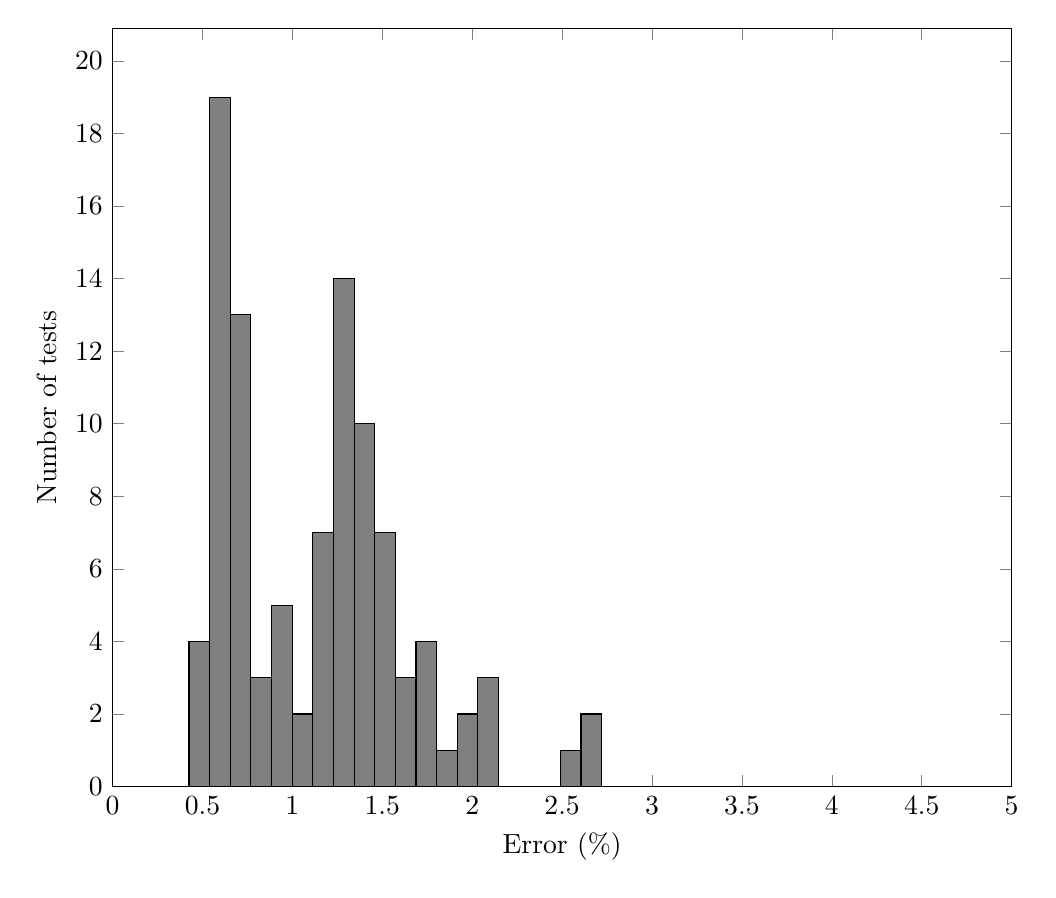
\begin{tikzpicture}
  \begin{axis}[
    width=13cm,
    ylabel=Number of tests,
    xlabel=Error (\%),
    xmin=0,xmax=5,ymin=0,]
    \addplot [ybar interval,fill=gray,draw=black] coordinates {
(0.42510531,  4.)
(0.53985223, 19.)
(0.65459915, 13.)
(0.76934608,  3.)
(0.884093,  5.)
(0.99883992,  2.)
(1.11358684,  7.)
(1.22833377, 14.)
(1.34308069, 10.)
(1.45782761,  7.)
(1.57257453,  3.)
(1.68732146,  4.)
(1.80206838,  1.)
(1.9168153, 2.)
(2.03156222,  3.)
(2.14630914,  0.)
(2.26105607,  0.)
(2.37580299,  0.)
(2.49054991,  1.)
(2.60529683,  2.)
(2.72004376,  0.)
    };
  \end{axis}
\end{tikzpicture}